\documentclass[12pt,a4paper]{article}
\usepackage[russian]{babel}
\usepackage[utf8]{inputenc}
\usepackage{mathtools}
\usepackage{amsfonts}
\usepackage{amssymb}
\usepackage{enumitem}
\usepackage{alltt}
\usepackage{graphicx}
\usepackage{indentfirst}
\usepackage{caption}
\usepackage{float}
\usepackage{wrapfig}
\setlength{\parindent}{0.75cm}
\graphicspath{{pictures/}}
\DeclareGraphicsExtensions{.png}
\usepackage[left=15mm,right=15mm,top=2cm,bottom=2cm]{geometry}
\author{Глотов Алексей}
\begin{document}
\newpage
\begin{center}
\footnotesize{{ГОСУДАРСТВЕННОЕ АВТОНОМНОЕ ОБРАЗОВАТЕЛЬНОЕ УЧРЕЖДЕНИЕ}\break
{ВЫСШЕГО ОБРАЗОВАНИЯ}
\break
{\bf {МОСКОВСКИЙ ФИЗИКО-ТЕХНИЧЕСКИЙ ИНСТИТУТ}}
\break
\small{(НАЦИОНАЛЬНЫЙ ИССЛЕДОВАТЕЛЬСКИЙ УНИВЕРСИТЕТ)}}
\break
\hfill \break
\hfill \break
\begin{center}
\normalsize{Кафедра общей физики}
\end{center}
\hfill \break
\hfill \break
\hfill \break
\hfill \break

\begin{center}
\normalsize {Лабораторная работа 1.4.5}
\end{center}
\hfill \break\\
\large{Изучение колебаний струны}
\end{center}
\begin{flushleft}
\hfill \break
\hfill \break
\hfill \break
\hfill \break
\hfill \break
\hfill \break
\hfill \break
\hfill \break
\hfill \break
\hfill \break
\hangindent=9cm
\normalsize{Преподаватель:}\hfill
\normalsize{к.ф.-м.н., доц. Яворский В.А.}\\
\hfill \break
\normalsize{Обучающийся:}\hfill
\normalsize{Глотов А.А} \\
\hfill \break
\end{flushleft}
\hfill \break
\hfill \break
\hfill \break
\hfill \break
\hfill \break
\hfill \break
\hfill \break
\hfill \break
\hfill \break
\hfill \break
\hfill \break

\begin{center}
Долгопрудный \break
 2021
\end{center}
\thispagestyle{empty}
\newpage
\begin{center}
\large{\bf Введение} 
\end{center}
\begin{center}
\large{Цели работы} \break
\end{center}
\begin{itemize}
\item Исследование зависимости частоты колебаний струны от величины натяжения
\item Исследование условий установления стоячей волны
\end{itemize}
\hfill \break
\begin{center}
\large{Приборы и материалы}
\end{center}
\begin{enumerate}
\item Рейка со струной
\item Звуковой генератор
\item Постоянный магнит
\item Разновесы
\end{enumerate}
\begin{center}
\large Теоретические сведения
\end{center}
\par Основное свойство струны - гибкость - является следствием ее большой длины по сравнению с поперечными размерами, что позволяет нам пренебречь величиной изгибных напряжений.
\par При приложении силы вдоль струны к двум ее концам, струна вытягивается в прямую линию. Сила натяжения при этом значительно больше ее силы тяжести, что позволяет нам ей пренебречь.
\par Движение элементов струны может быть вызвано изменением ее формы или придаче ей импульса. Натяжение струны стремится вернуть струну к исходному состоянию, из-за чего возникают колебания в струне.
\par Известно, что скорость распространения поперечной волны на струне равна 
\begin{equation}
u=\sqrt{\frac{F}{\rho}}
\end{equation} 
где $\rho$ - линейная плотность струны
\par Для всех типов волн справедливо соотношение 
\begin{equation}
\lambda=\frac{u}{\nu}
\end{equation}
где $\nu$ - частота колебаний струны - определяется по формуле 
\begin{equation}
\nu=n\frac{u}{2l} = \frac{n}{2l}\sqrt{\frac{F}{\rho}}
\end{equation}
l - длина струны, n - число полуволн
\begin{figure}[H]
\centering
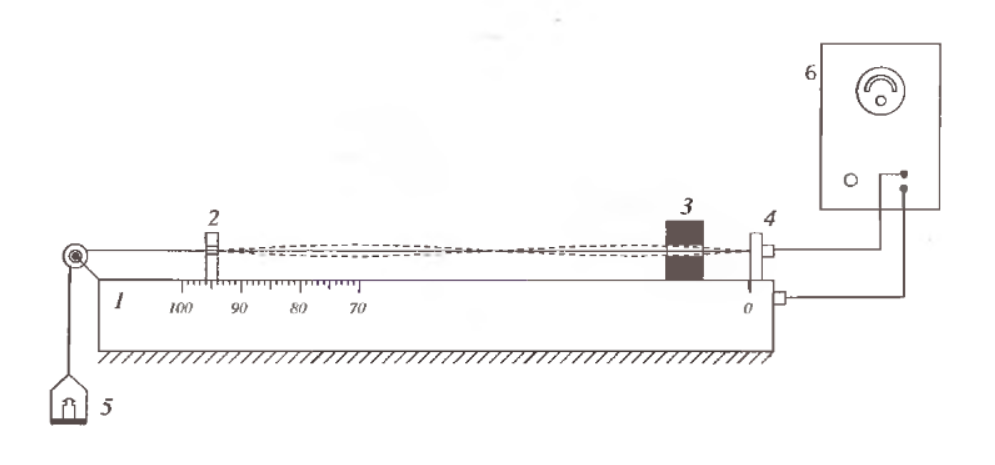
\includegraphics[width=14cm, height=7cm]{1.4.5_1}
\caption{Схема экспериментальной установки}
\label{pic:1}
\end{figure}

\par На рисунке цифрами обозначены:
\begin{enumerate}
\item - металлическая рейка
\item - подвижная опора
\item - подвижный магнит
\item - неподвижная опора
\item - чашка для грузов
\item - звуковой генератор
\end{enumerate}
\par В представленной установке движение струны вызывается силой Ампера, действующей на проводник с током, т.е. струну. Частота колебаний равна частоте колебания тока в струне, т.е. частоте, выставленной на генераторе. В натянутой струне возникают колебания и по ней побегут волны, отражающиеся от опор и, складываясь друг с другом, создают стоячую волну, если на струне уложатся целое число полуволн.
\par Из-за потерь энергии в системе, необходимо постоянно подводить энергию к колеблющейся струне так, чтобы полная энергия системы оставалась постоянной.
\par Необходимо также отметить, что в стоячей волне невозможно распространение энергии, что в неидеальных условиях приводит к размытию узлов нашей стоячей волны. Введем коэффициент бегучести, определяемый по формуле
\begin{equation}
\frac{A_{1} - A_{2}}{A_{2}}
\end{equation}
$A_{1}$ - амплитуда падающей волны, $A_{2}$  -амплитуда отраженной волны. В случае, если коэффициент бегучести значительно меньше единицы, волну можно считать чисто стоячей. Величину $A_{1} - A_{2}$ можно оценить по размытию узлов стоячей волны - она равна половине значения величины размытия. Амплитуда стоячей волны в пучности равна $2A_{2}$
\newpage
\begin{center}
\large Ход работы
\end{center}
1) \par Запишем характеристики исследуемой струны \hfill \break
M - масса подвеса \hfill \break
d - диаметр проволоки \hfill \break
$\rho_{l}$ - линейная плотность струны \hfill \break
M =  952.9 г \;\;\;\;\; $\Delta_{M}$ = 1 г (тройная погрешность, т.к. подвес состоит из чашки и двух грузов) \hfill \break
$\rho_{l} = 0.568 \frac{\text{г}}{\text{м}}$  \hfill \break
\par По этим данным по (2) оценим скорость распространения волны без дополнительных грузов \hfill \break
$u = 128.2 \frac{\text{м}}{с}$  
$\sigma_{u}=u\sqrt{0.25(\frac{\Delta_{M}}{M})^2+0.25(\frac{\Delta_{\rho}}{\rho})^2 + 0.25(\frac{\Delta_{g}}{g})^2} = 0.1\frac{\text{м}}{с}$ \hfill \break
\par Посчитаем частоту основной гармоники $\nu_{1}$ \hfill \break
$\nu_{1} = 128.8 \text{Гц}$ \hfill \break
$\sigma_{\nu} = \nu\sqrt{0.25(\frac{\Delta_{M}}{M})^2+0.25(\frac{\Delta_{\rho}}{\rho})^2+0.25(\frac{\Delta_{g}}{g})^2+(\frac{\Delta_{L}}{L})^2} = 0.3\text{Гц}$ \hfill \break
2) \par Пронаблюдаем стоячие волны при различных значениях и запишем получившиеся значения частоты на генераторе в таблицу. \hfill \break
\begin{center}
\begin{tabular}{|c|c|c|c|c|c|c|c|}
 \hline 
 n & 1 & 2 & 3 & 4 & 5 & 6 & 7 \\ 
 \hline 
 $\nu$, \text{Гц} & 122,8 & 244,9 & 382,6 & 491,1 & 633,7 & 736,8 & 870,6 \\ 
 \hline 
\end{tabular}  
\end{center}
3) \par Проведем измерения частот стоячей волны струны при заданных натяжении и длине. Сначала - для нечетных гармоник, после - для четных, сдвигая регистрирующий датчик в точки пучности волны. Занесем данные в таблицу. Повторим измерения для различных масс \hfill \break
\begin{center}
\begin{tabular}{|c|c|c|c|c|c|}
\hline 
m, \text{г} & 331.0 & 493,2 & 824,2 & 1288,3 & 1778,4 \\ 
\hline 
n & \multicolumn{5}{c|}{$\nu$, \text{Гц}} \\ 
\hline 
1 & 147,9 & 156,3 & 175,4 & 197,1 & 217,5 \\ 
\hline 
2 & 297,0 & 316,6 & 350,9 & 395,1 & 434,3 \\ 
\hline 
3 & 448,3 & 469,3 & 526,9 & 592,1 & 652,7 \\ 
\hline 
4 & 597,5 & 628,9 & 702,2 & 789,1 & 869,7 \\ 
\hline 
5 & 745,2 & 783,0 & 879,4 & 985,9 & 1087,9 \\ 
\hline 
6 & 888,4 & 949,8 & 1053,0 & 1184,0 & 1304,7 \\ 
\hline 
7 & 1048,3 & 1099,1 & 1228,5 & 1380,0 & 1521,8 \\ 
\hline 
8 & 1189,7 & 1258,3 & 1403,4 & 1572,8 & 1746,0 \\ 
\hline 
9 & 1351,5 & 1408,5 & 1580,2 & 1774,5 & - \\ 
\hline 
\end{tabular}
\end{center}
\newpage
4)  По данным, полученным в п.4 построим графики $\nu(n)$
\begin{center}
\begin{figure}[H]
\centering
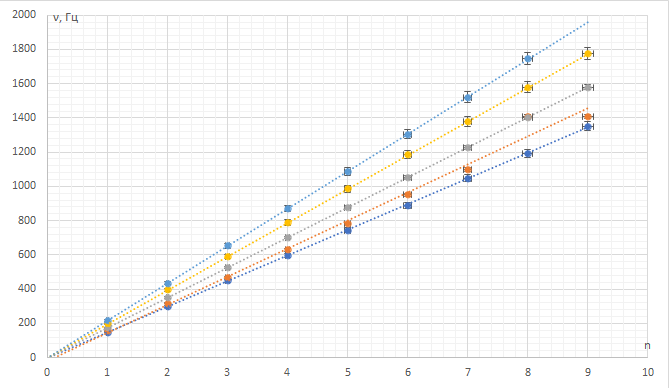
\includegraphics[width=15cm, height=9cm]{1.4.5_gr_1}
\caption{График зависимости $\nu(n)$}
\label{gr:1}
\end{figure}
\end{center}
\par По МНК определим значение углов наклона наших прямых \hfill \break
\large $\alpha = \frac{<\nu{n}>}{<n^2>}$  \hfill \hfill \break
$\sigma_{\alpha}=\sqrt{\frac{1}{n - 1}(\frac{<y^2>}{<x^2>} - (\alpha)^2)}$
\hfill \break
$\alpha_{1}=149.7\text{Гц}$ \;\;\;\;\; $\sigma_{\alpha_{1}}=0.3\text{Гц}$ \hfill \break
$\alpha_{2}=156.8\text{Гц}$ \;\;\;\;\; $\sigma_{\alpha_{2}}=0.2\text{Гц}$ \hfill \break
$\alpha_{3}=175.5\text{Гц}$ \;\;\;\;\; $\sigma_{\alpha_{3}}=0.1\text{Гц}$ \hfill \break
$\alpha_{4}=197.2\text{Гц}$ \;\;\;\;\; $\sigma_{\alpha_{4}}=0.1\text{Гц}$ \hfill \break
$\alpha_{5}=218.0\text{Гц}$ \;\;\;\;\; $\sigma_{\alpha_{5}}=0.2\text{Гц}$ \hfill \break
5) По формулам (1) и (3) видно, что $u = 2l\alpha$ \hfill \break
l = 0.5 м \;\;\;\;\; $\Delta{l} = 0.001$м \hfill \break
Тогда пересчитаем значения коэффициентов наклона в скорости распространения волны в струне
\begin{center}
\begin{tabular}{|c|c|c|c|c|c|}
  \hline 
  $\alpha$, \text{Гц} & 149.7 & 156.8 & 175.5 & 197.2 & 218.0 \\ 
  \hline 
  u, $\frac{\text{м}}{c}$ & 149.7 & 156.8 & 175.5 & 197.2 & 218.0 \\ 
  \hline
  $u^2, \frac{\text{м}^2}{c^2}$ & 22410 & 24586 & 30800 & 38887 & 47524 \\
  \hline 
\end{tabular} 
\end{center}
6) Построим по полученным данным график зависимости $u^2(T)$
\begin{center}
\begin{figure}[H]
\centering
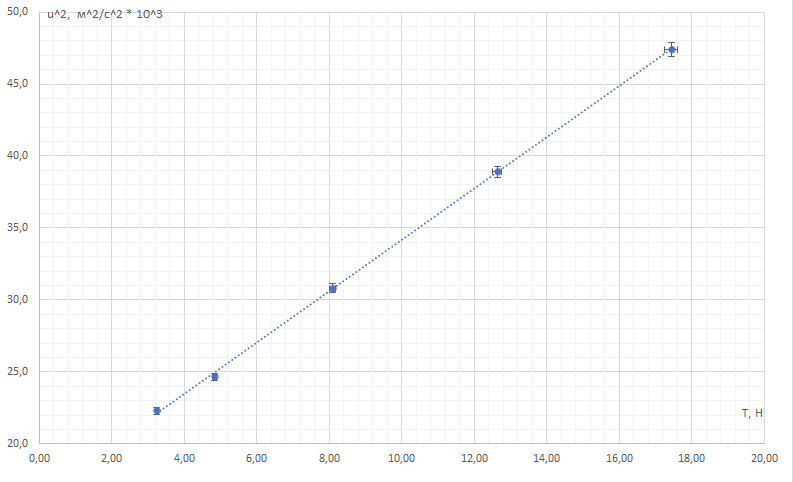
\includegraphics[width=15cm, height=9cm]{1.4.5_gr_2}
\caption{График зависимости $u^2(T)$}
\label{gr:2}
\end{figure}
\end{center}
$\beta=\frac{<u^2T>-<u^2><T>}{<T^2>-<T>^2}=1,78*10^3\frac{\text{м}}{\text{кг}}$ \hfill \break
$\sigma_{\beta}=\sqrt{\frac{1}{3}(\frac{<u^4>-<u^2>^2}{<T^2>-<T>^2}}*1,2=0.02*10^3\frac{\text{м}}{\text{кг}}$ \hfill \break
где 1,2 - коэффициент Стьюдента для 5 измерений \hfill \break
По углу наклона графика определим линейную плотность струны \hfill \break
$u^2=\frac{1}{\rho}T$, значит $\rho=\frac{1}{\beta}$\hfill \break
$\rho=5.62*10^{-4}\frac{\text{кг}}{\text{м}}$
\hfill \break
$\sigma_{\rho}=\sqrt{(\sigma^{\text{приб}}_{\rho})^2+(\sigma^{\text{случ}}_{\rho})^2}$ \hfill \break
$\sigma^{\text{случ}}_{\rho}=\rho\frac{\sigma_{\beta}}{\beta}$ \hfill \break
$(\sigma^{\text{приб}}_{\rho})^2=\rho^2(4(\frac{\sigma_{u}}{u})^2+(\frac{\sigma_{T}}{T})^2=4(\frac{\Delta{l}}{l})^2+4(\frac{\Delta{\nu}}{\nu})^2+(\frac{\Delta{m}}{m})^2+(\frac{\Delta{g}}{g})^2)$ \hfill \break
$\sigma_{\rho}=0,07*10^{-4}\frac{\text{кг}}{\text{м}}$ \hfill \break
7) Установим на генераторе частоту $\nu=\frac{\nu_{1}}{2}$ и пронаблюдаем картину, появившуюся на экране осциллографа 
\begin{center}
\begin{figure}[H]
\centering
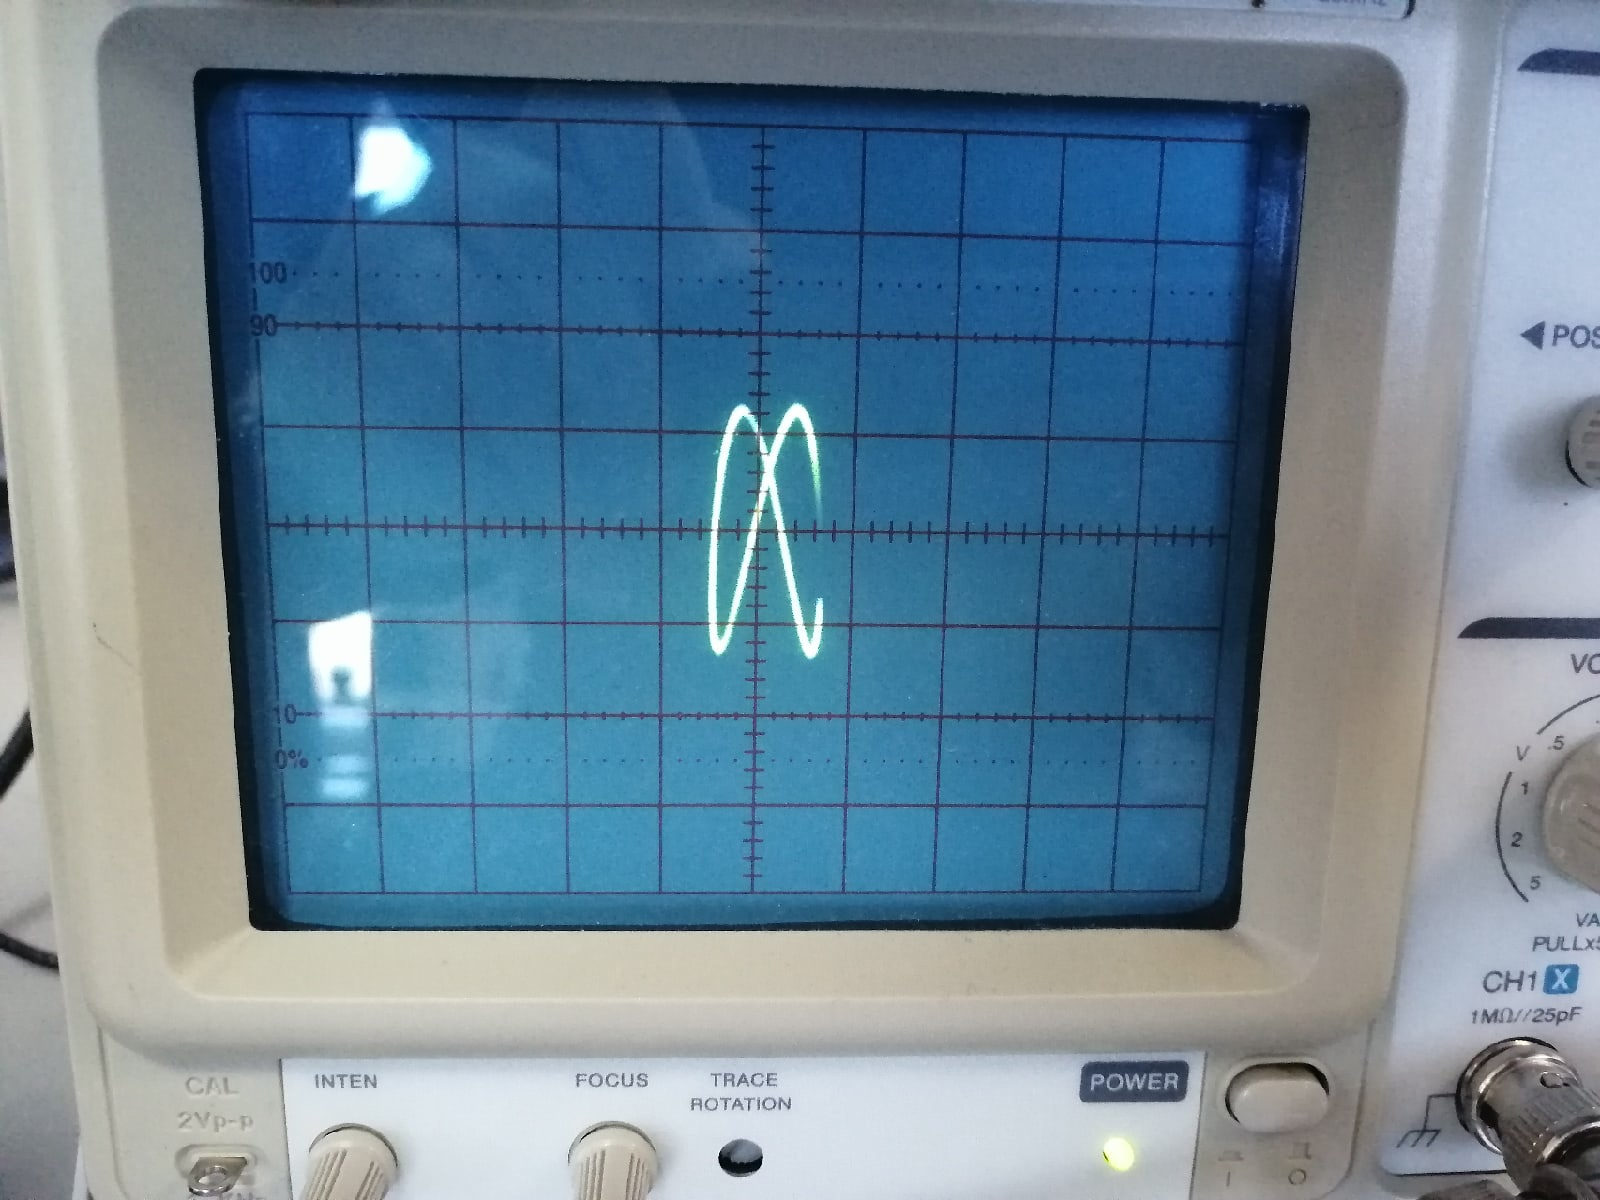
\includegraphics[width=15cm, height=9cm]{1.4.5_2}
\caption{Экран осциллографа}
\label{gr:2}
\end{figure}
\end{center}
\par Картинка на экране осциллографа соответствует фигуре Лиссажу, появляющейся при отношении частот 1:2. Значит, отношение частот на датчике (то есть и на исследуемом участке струны) и генераторе частоты отличаются как 1/2.
\newpage
\begin{center}
\large Выводы
\end{center}
\par В ходе экспериментов было показано существование стоячих волн в струне и продемонстрировано это на практике
\par В ходе работы были подтверждены теоретические зависимости. С точностью 0,2\% подтверждена формула для определения частоты первой гармоники струны. С точностью не более 0,2\% была подтверждена формула для определения скорости распространения волны в струне.
\par С точностью 1.3\% было получено значение линейной плотности струны $\rho=(5.62\pm0.07)*10^{-4} \frac{\text{кг}}{\text{м}}$, что совпадает со значением, приведенным на установке (0.568$\frac{\text{г}}{\text{м}})$
\end{document}